\documentclass[../notes.tex]{subfiles}

\pagestyle{main}
\renewcommand{\chaptermark}[1]{\markboth{\chaptername\ \thechapter\ (#1)}{}}

\begin{document}




\chapter{The Molecular Level}
\section{Chemical Biology Introduction and the Central Dogma}
\begin{itemize}
    \item \marginnote{9/27:}Questions:
    \begin{itemize}
        \item What edition(s) of the textbook(s) should we have?
        \begin{itemize}
            \item Doesn't matter.
        \end{itemize}
        \item Will there be TA office hours?
        \begin{itemize}
            \item No.
        \end{itemize}
    \end{itemize}
    \item CHEM 233 used to be Intermediate Organic Chemistry, and CHEM 332 was the grad class. They have been merged this year because of the overlap in content.
    \item Krishnan weeks 5-7; Tang otherwise.
    \item We will not be going through reactions. The format is slides; don't try to copy them down, just make some notes. Copy them down ahead of time!
    \item Goes over the syllabus.
    \begin{itemize}
        \item No fixed textbook. Lehninger is recommended though. Whatever edition you can find.
        \item No office hours (ask questions in class or ask her to meet outside).
        \begin{itemize}
            \item Tang will show up early and stay late.
        \end{itemize}
        \item Midterms are 1 hour; final is 2 hours.
        \item Three problem sets.
        \item One in-class quiz:
        \begin{itemize}
            \item Krishnan will give us cutting-edge literature to read one week before the quiz and 5 questions.
            \item We can form study groups to discuss the questions.
            \item Multiple choice quiz on that day.
        \end{itemize}
        \item We're not supposed to memorize things in this course; the problems won't be like that.
        \item Tang may lower the exam difficulty levels from previous years.
        \item Tang doesn't want us to have to fight for points; is trying to give us a big curve so that we can just focus on learning.
        \item Since this is now only a twice a week class, Tang is cutting material on carbohydrates and protein design. May try to squeeze in orthogonal chemistry, though.
    \end{itemize}
    \item The central dogma in biology.
    \emph{picture}
    \begin{itemize}
        \item DNA $\to$ RNA $\to$ protein $\to$ needed chemical transformations.
    \end{itemize}
    \item Size in biology.
    \begin{itemize}
        \item An activity matching biological entities (e.g., E. coli, cells, RNA) to their sizes in microns.
        \item Uses the world zoom website.
        \item We may be tested on sizes, but only relative not exact (e.g., E. coli vs. a ribosome).
    \end{itemize}
    \item Red blood cells are smaller than normal cells because they don't have nuclei, and they don't need meat to divide.
    \item Concentrations in biology.
    \begin{figure}[h!]
        \centering
        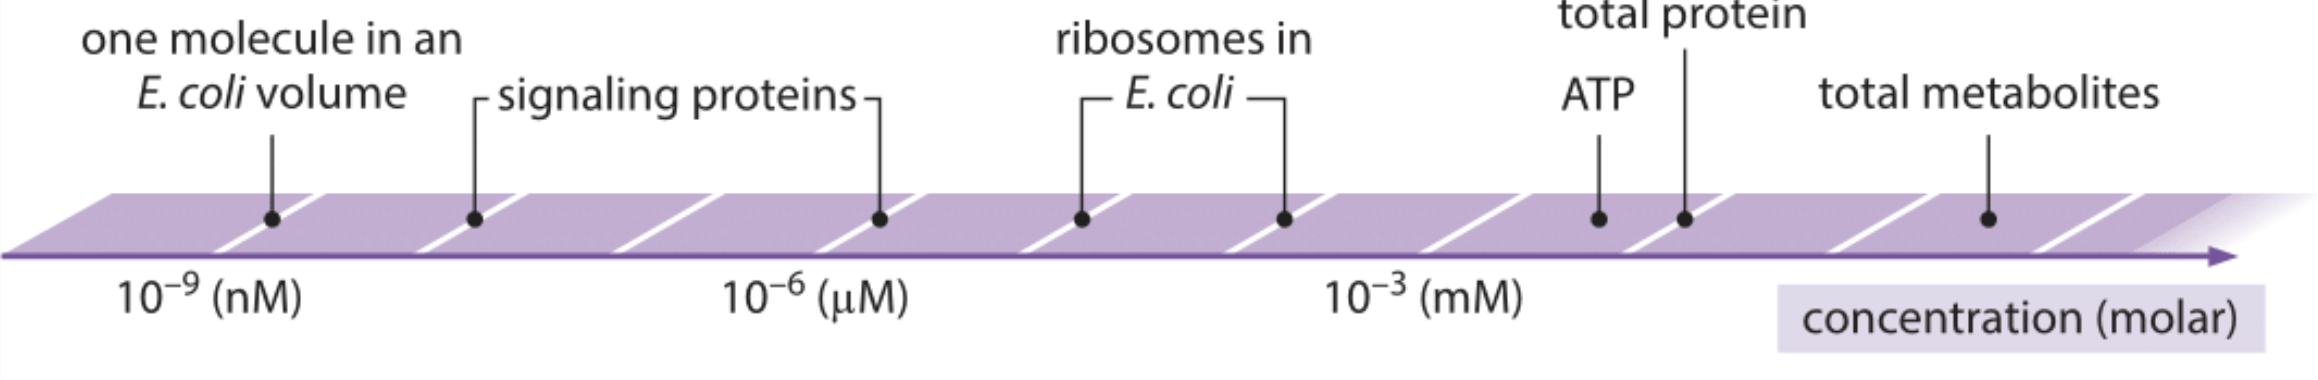
\includegraphics[width=0.9\linewidth]{../ExtFiles/bioConcentrations.png}
        \caption{Concentrations in biology.}
        \label{fig:bioConcentrations}
    \end{figure}
    \begin{itemize}
        \item You need a couple of copies of signaling proteins.
        \item Cells dedicate a lot of resources to building ribosomes.
        \item Different ions have different concentrations in different parts of the body. Additionally, different types of cells have different concentrations.
    \end{itemize}
    \item \emph{Bound} divalent ions such as \ce{Mg^2+} help cancel the charge of ATP; that's why we need them in solution.
    \item The materials left after we remove all of the water from our cells.
    \begin{itemize}
        \item Largely protein, lipid, rRNA.
        \item Far more mRNA and proteins in mammalian cells than bacterial cells.
    \end{itemize}
    \item Time for protein diffusion within a cell.
    \begin{itemize}
        \item Time scale $\tau$ to traverse distance $R$ given diffusion coefficient $D$:
        \begin{equation*}
            \tau = \frac{R^2}{6D}
        \end{equation*}
        \item For a protein in cytoplasm, $D\approx\SI[per-mode=symbol]{10}{\square\micro\meter\per\second}$.
    \end{itemize}
    \item The molecular hierarchy of structure.
    \begin{itemize}
        \item The cell and its organelles are made of supramolecular complexes (e.g., the plasma membrane, chromatin, and the cell wall), which are made up of macromolecules (e.g., DNA, proteins, cellulose), which are made up of monomeric units (e.g., nucleotides, amino acids and sugars).
    \end{itemize}
    \item We will be expected to know how to draw the amino acids and nucleic acid bases.
    \item We will not talk much about lipids and sugars.
    \item Chirality and isomers review.
    \item Thalidomide.
    \begin{itemize}
        \item Was only distributed in Germany; the FDA is very proud of having picked up on the scientific malpractice and barred it from ever entering the US.
        \item Just selling one isomer doesn't work because it racemizes so quickly.
        \item Now used to treat cancer; you have to sign a bunch of paperwork saying that you won't get pregnant before you use it.
    \end{itemize}
\end{itemize}



\section{Chemistry and Biophysics of Nucleic Acids}
\begin{itemize}
    \item \marginnote{9/29:}Feel free to come by and introduce yourself now that the class is a more manageable size.
    \item DNA and RNA basics.
    \item Humans have on the order of \num{3e13} cells and on the order of \SI{1}{\meter} of DNA in each cell.
    \begin{itemize}
        \item Calculated by multiplying the number of base pairs per cell ($\approx\num{3e9}$) by the length of each base pair ($\approx\SIrange{3.3}{3.4}{\angstrom}$).
        \item Some people say \SI{2}{\meter} because we have two copies of our genome.
        \item DNA wraps around histone proteins to form chromosomes to fit into such a tiny space.
    \end{itemize}
    \item DNA is ACTG. RNA is ACUG.
    \item \textbf{Bases} and their corresponding \textbf{nucleosides}.
    \begin{figure}[h!]
        \centering
        \footnotesize
        \begin{subfigure}[b]{0.19\linewidth}
            \centering
            \chemfig{*6(-N=-N=(-NH_2)-(*5(-N=-[,,,2]HN-))=)}
            \caption{Adenine.}
            \label{fig:baseNucleosidea}
        \end{subfigure}
        \begin{subfigure}[b]{0.19\linewidth}
            \centering
            \chemfig{*6(-N=(-NH_2)-NH-(=O)-(*5(-N=-[,,,2]HN-))=)}
            \caption{Guanine.}
            \label{fig:baseNucleosideb}
        \end{subfigure}
        \begin{subfigure}[b]{0.19\linewidth}
            \centering
            \chemfig{*6(-\chembelow{N}{H}-(=O)-NH-(=O)-(-H_3C)=)}
            \vspace{1em}
            \caption{Thymine.}
            \label{fig:baseNucleosidec}
        \end{subfigure}
        \begin{subfigure}[b]{0.19\linewidth}
            \centering
            \chemfig{*6(-\chembelow{N}{H}-(=O)-N=(-NH_2)-=)}
            \vspace{1em}
            \caption{Cytosine.}
            \label{fig:baseNucleosided}
        \end{subfigure}
        \begin{subfigure}[b]{0.19\linewidth}
            \centering
            \chemfig{*6(-\chembelow{N}{H}-(=O)-NH-(=O)-=)}
            \vspace{1em}
            \caption{Uracil.}
            \label{fig:baseNucleosidee}
        \end{subfigure}
        \begin{subfigure}[b]{0.33\linewidth}
            \centering
            \chemfig{*6(-N=-N=(-NH_2)-(*5(-N=-N(-?<[:-110]@{C2}-[4,,,,line width=2pt]@{C3}(-[:-130]HO)>[:110](-[:25,0.93]O?)(-[:108]-[::60]HO))-))=)}
            \chemmove{
                \fill ([xshift=0.1pt]C2) circle (1pt);
                \fill ([xshift=-0.1pt]C3) circle (1pt);
            }
            \caption{Deoxyadenosine.}
            \label{fig:baseNucleosidef}
        \end{subfigure}
        \begin{subfigure}[b]{0.32\linewidth}
            \centering
            \chemfig{*6(-N=(-NH_2)-NH-(=O)-(*5(-N=-N(-?<[:-110]@{C2}-[4,,,,line width=2pt]@{C3}(-[:-130]HO)>[:110](-[:25,0.93]O?)(-[:108]-[::60]HO))-))=)}
            \chemmove{
                \fill ([xshift=0.1pt]C2) circle (1pt);
                \fill ([xshift=-0.1pt]C3) circle (1pt);
            }
            \caption{Deoxyguanosine.}
            \label{fig:baseNucleosideg}
        \end{subfigure}\\[2em]
        \begin{subfigure}[b]{0.33\linewidth}
            \centering
            \chemfig{*6(-N(-[:-108]?<[:-110]@{C2}-[4,,,,line width=2pt]@{C3}(-[:-130]HO)>[:110](-[:25,0.93]O?)(-[:108]-[::60]HO))-(=O)-NH-(=O)-(-H_3C)=)}
            \chemmove{
                \fill ([xshift=0.1pt]C2) circle (1pt);
                \fill ([xshift=-0.1pt]C3) circle (1pt);
            }
            \caption{Deoxythymidine.}
            \label{fig:baseNucleosideh}
        \end{subfigure}
        \begin{subfigure}[b]{0.32\linewidth}
            \centering
            \chemfig{*6(-N(-[:-108]?<[:-110]@{C2}-[4,,,,line width=2pt]@{C3}(-[:-130]HO)>[:110](-[:25,0.93]O?)(-[:108]-[::60]HO))-(=O)-N=(-NH_2)-=)}
            \chemmove{
                \fill ([xshift=0.1pt]C2) circle (1pt);
                \fill ([xshift=-0.1pt]C3) circle (1pt);
            }
            \caption{Deoxycytidine.}
            \label{fig:baseNucleosidei}
        \end{subfigure}
        \begin{subfigure}[b]{0.33\linewidth}
            \centering
            \chemfig{*6(-N(-[:-108]?<[:-110]@{C2}-[4,,,,line width=2pt]@{C3}(-[:-130]HO)>[:110](-[:25,0.93]O?)(-[:108]-[::60]HO))-(=O)-NH-(=O)-=)}
            \chemmove{
                \fill ([xshift=0.1pt]C2) circle (1pt);
                \fill ([xshift=-0.1pt]C3) circle (1pt);
            }
            \vspace{1em}
            \caption{Uridine.}
            \label{fig:baseNucleosidej}
        \end{subfigure}
        \caption{Bases and nucleosides.}
        \label{fig:baseNucleoside}
    \end{figure}
    \begin{itemize}
        \item Notice that deoxyribose is joined with the base at its $2'$ carbon.
        \item If we use ribose instead of deoxyribose, we get adenosine, guanosine, etc.
        \item Memorize these structures!
    \end{itemize}
    \item Nomenclature.
    \item \textbf{Base}: The heterocycle. \emph{Also known as} \textbf{nucleobase}.
    \item \textbf{Ribose}: A 5-carbon monosaccharide, a derivative of which is a component of DNA.
    \item \textbf{Deoxyribose}: A molecule identical to ribose but without the $2'$ hydroxyl group.
    \begin{figure}[H]
        \centering
        \footnotesize
        \begin{subfigure}[b]{0.2\linewidth}
            \centering
            \chemfig{CH_2OH-[6]?<[:-60]@{C3}(-[6]OH)-[,,,,line width=2pt]@{C2}(-[6]OH)>[:60](-[2]OH)-[:155,1.1]O?}
            \chemmove{
                \fill ([xshift=0.1pt]C2) circle (1pt);
                \fill ([xshift=-0.1pt]C3) circle (1pt);
            }
            \caption{Ribose.}
            \label{fig:dnaSugarsa}
        \end{subfigure}
        \begin{subfigure}[b]{0.2\linewidth}
            \centering
            \chemfig{CH_2OH-[6]?<[:-60]@{C3}(-[6]OH)-[,,,,line width=2pt]@{C2}>[:60](-[2]OH)-[:155,1.1]O?}
            \chemmove{
                \fill ([xshift=0.1pt]C2) circle (1pt);
                \fill ([xshift=-0.1pt]C3) circle (1pt);
            }
            \caption{Deoxyribose.}
            \label{fig:dnaSugarsb}
        \end{subfigure}
        \caption{DNA sugars.}
        \label{fig:dnaSugars}
    \end{figure}
    \item \textbf{Nucleoside}: Base + sugar.
    \item \textbf{Nucleotide}: Base + sugar + phosphate(s).
    \item Base numbering.
    \begin{figure}[h!]
        \centering
        \footnotesize
        \begin{subfigure}[b]{0.19\linewidth}
            \centering
            \chemfig{*6(-@{N3}N=-@{N1}N=@{C6}(-NH_2)-(*5(-@{N7}N=-[,,,2]H@{N9}N-))=)}
            \chemmove{
                \begin{scope}
                    \node [below left=-2pt of N1] {\tiny 1};
                    \node [above=0pt of N3] {\tiny 3};
                    \node [above left=-2pt of C6] {\tiny 6};
                    \node [below=0pt of N7,xshift=2pt] {\tiny 7};
                    \node [above=0pt of N9] {\tiny 9};
                \end{scope}
            }
            \caption{Adenine.}
            \label{fig:baseNumberinga}
        \end{subfigure}
        \begin{subfigure}[b]{0.19\linewidth}
            \centering
            \chemfig{@{C6}*6(-@{N1}\chembelow{N}{H}-@{C2}(=O)-@{N3}N=@{C4}(-NH_2)-@{C5}=)}
            \chemmove{
                \begin{scope}
                    \node [above=0pt of N1] {\tiny 1};
                    \node [above left=1pt of C2] {\tiny 2};
                    \node [below left=-4pt of N3] {\tiny 3};
                    \node [below=2pt of C4] {\tiny 4};
                    \node [below right=0pt of C5] {\tiny 5};
                    \node [above right=0pt of C6] {\tiny 6};
                \end{scope}
            }
            \vspace{1em}
            \caption{Cytosine.}
            \label{fig:baseNumberingb}
        \end{subfigure}
        \caption{Base numbering.}
        \label{fig:baseNumbering}
    \end{figure}
    \begin{itemize}
        \item Generalize from the above two examples.
    \end{itemize}
    \item Sugar numbering: Start to the right of the oxygen and move clockwise. Use primes do distinguish from the numbered base carbons.
    \begin{itemize}
        \item Remember that DNA and RNA run 5' to 3' with phosphate groups linking the deoxyribose groups.
    \end{itemize}
    \item Listing features common to all or some of the bases.
    \begin{itemize}
        \item E.g., heterocycles, on the way to being or already aromatic, nitrogen in the ring, oxygen only ever outside the ring, etc.
    \end{itemize}
    \item \textbf{Inosine}: An intermediate between adenine and guanine. \emph{Also known as} \textbf{hypoxanthine}. \emph{Structure}
    \begin{figure}[h!]
        \centering
        \footnotesize
        \chemfig{*6(-N=(-NH_2)-NH-(=O)-(*5(-N=-[,,,2]HN-))=)}
        \caption{Inosine.}
        \label{fig:inosine}
    \end{figure}
    \item Common modifications to adenine: Methylation at the 1 or 6 position.
    \item Five percent of cytosine exists in its methylated form; important epigenetically in determining which genes get turned on and off.
    \begin{itemize}
        \item Methylation of cytosine occurs at the 5-carbon.
    \end{itemize}
    \item Hydrogen bonding between bases.
    \begin{figure}[H]
        \centering
        \begin{subfigure}[b]{0.45\linewidth}
            \centering
            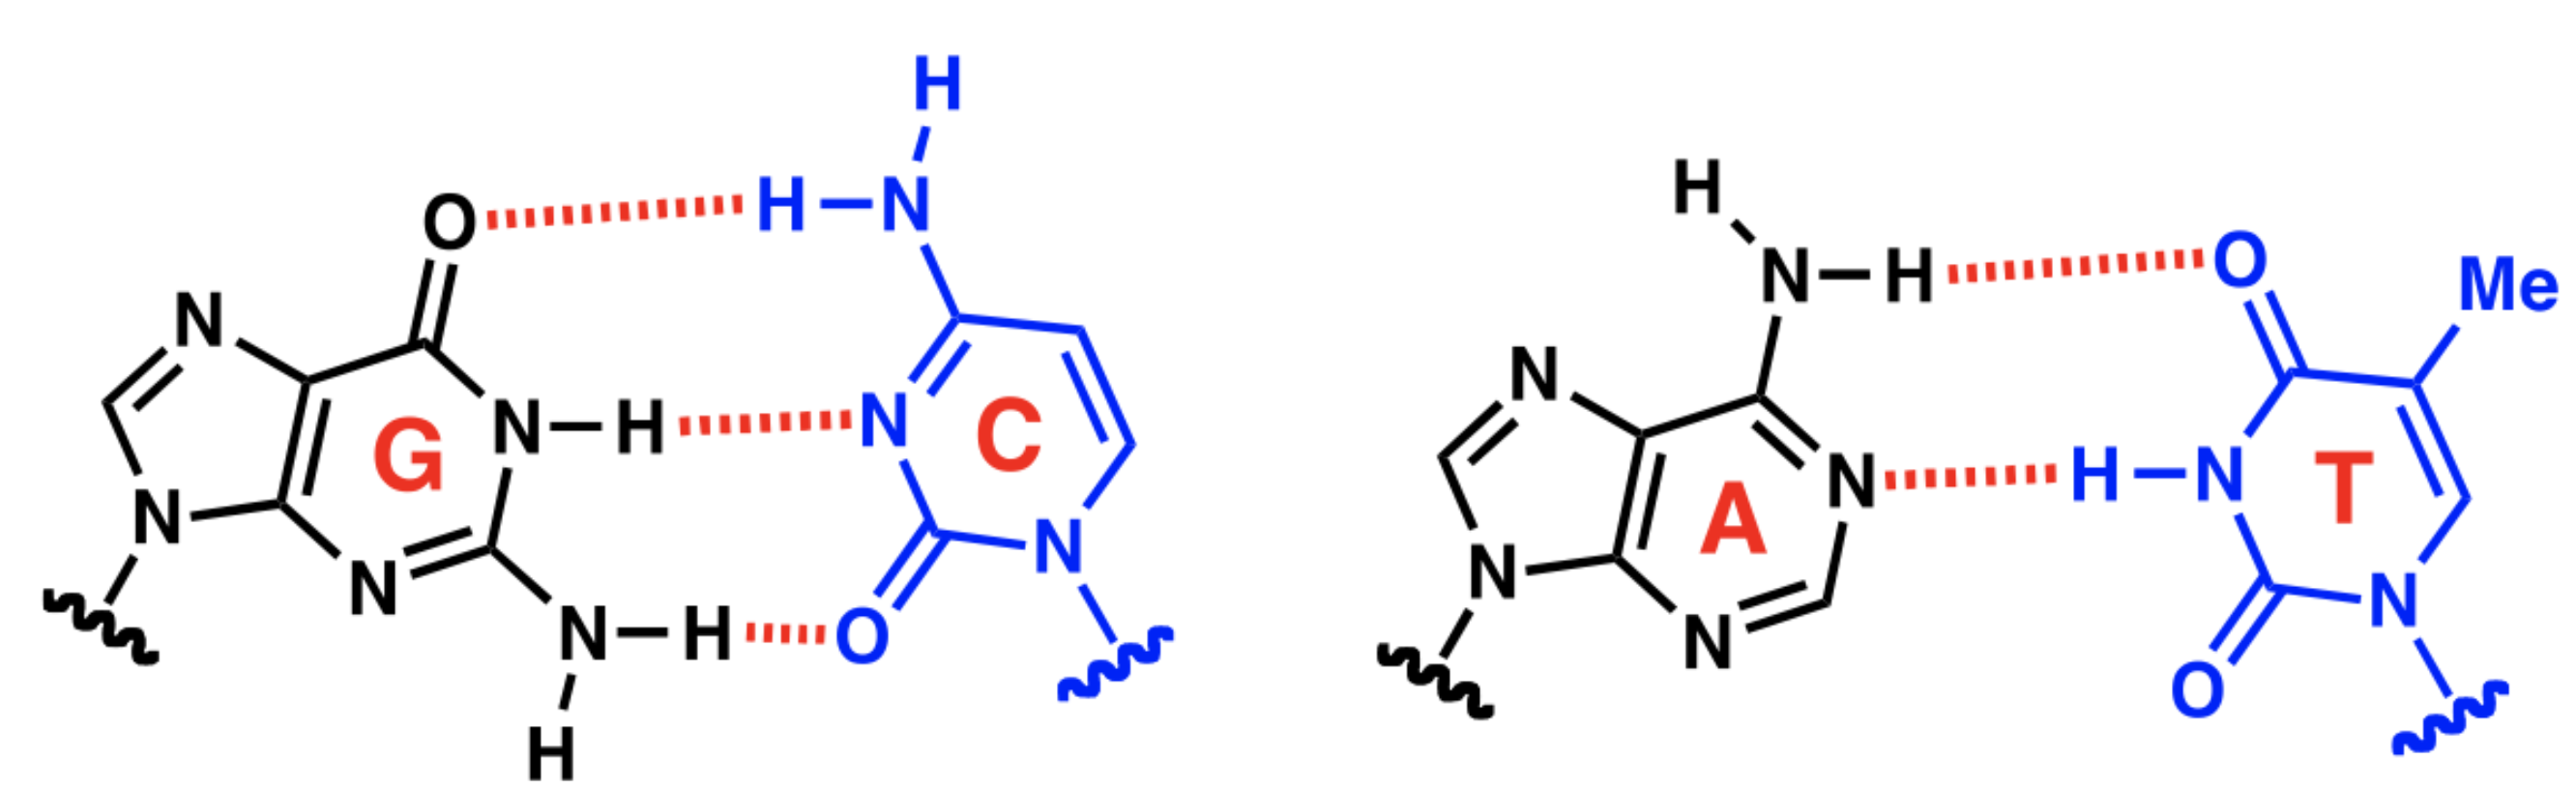
\includegraphics[width=\linewidth]{../ExtFiles/hBondinga.png}
            \caption{Watson-Franklin-Crick.}
            \label{fig:hBondinga}
        \end{subfigure}
        \begin{subfigure}[b]{0.45\linewidth}
            \centering
            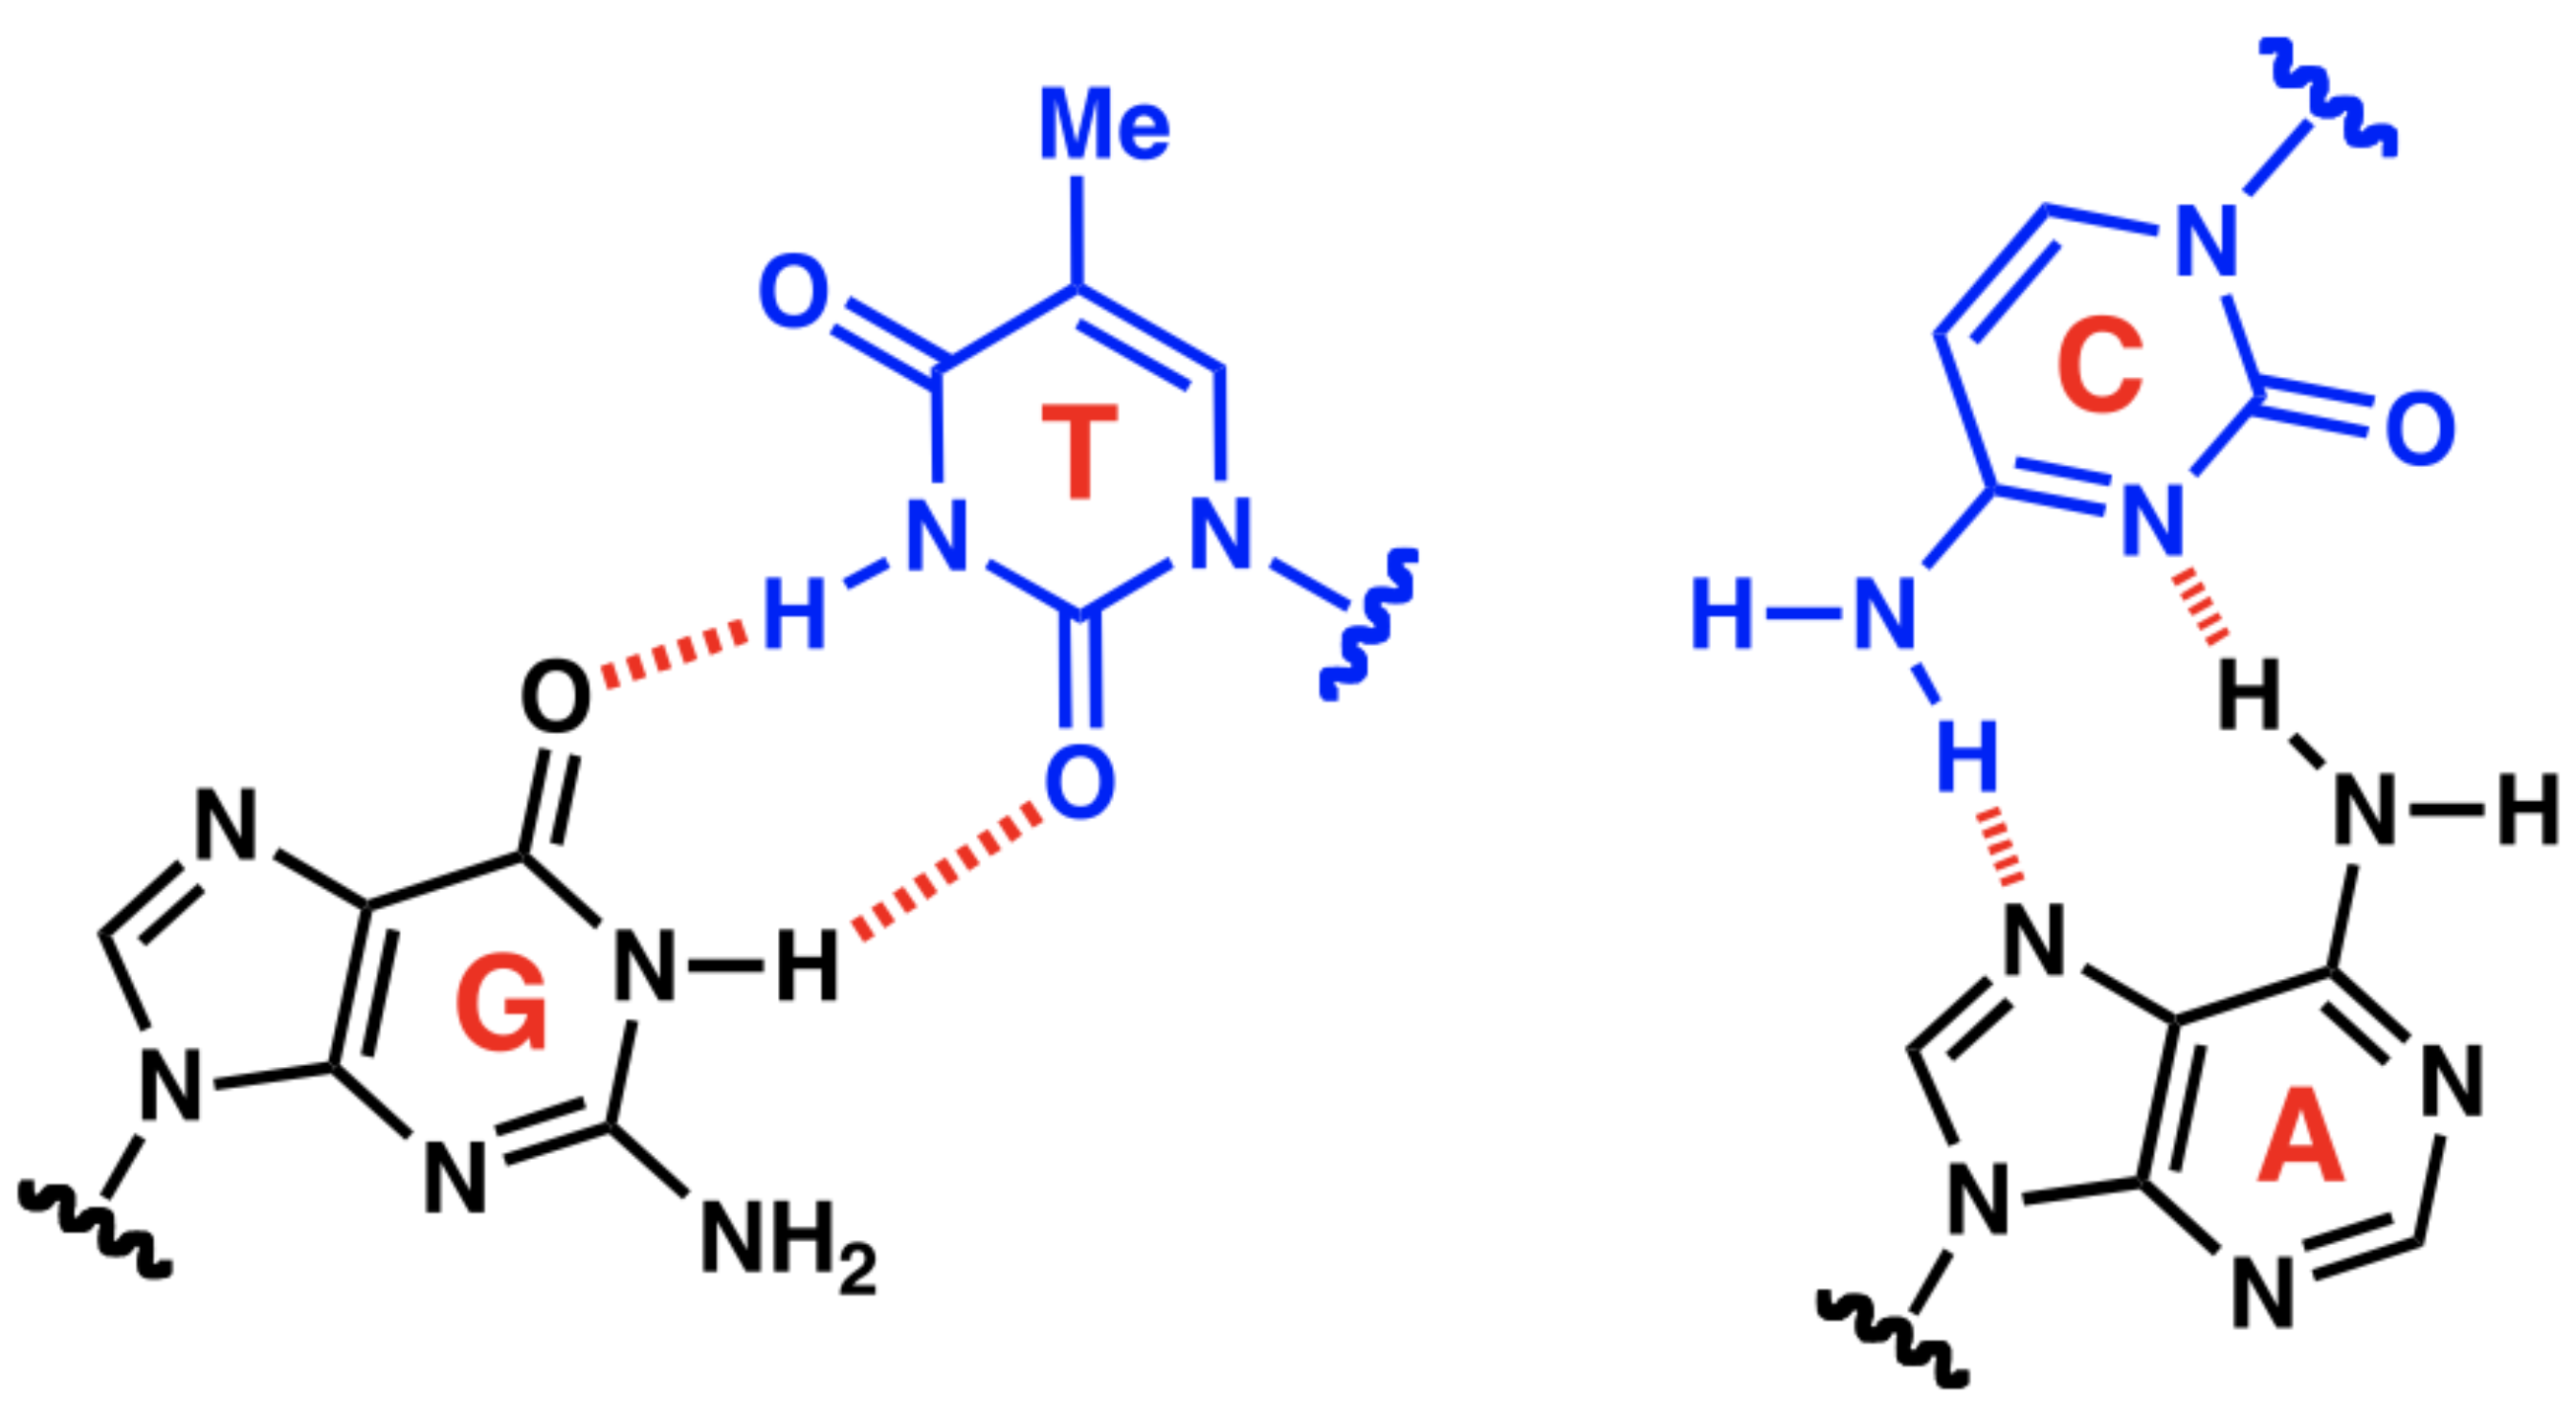
\includegraphics[width=0.8\linewidth]{../ExtFiles/hBondingb.png}
            \caption{Wobble.}
            \label{fig:hBondingb}
        \end{subfigure}
        \caption{Hydrogen bonding in bases.}
        \label{fig:hBonding}
    \end{figure}
    \begin{itemize}
        \item Hydrogen on a heteroatom serves as a donor; heteroatoms serve as acceptors.
        \item There are many types, but we're only responsible for Watson-Crick-Franklin and Wobble interactions.
        \item Watson-Crick-Franklin is the standard interaction found in double helix DNA.
        \item Wobble:
        \begin{itemize}
            \item G/T is more common and important than C/A in nature.
        \end{itemize}
    \end{itemize}
    \item A triplet codon NNN yields an amino acid. There are $4^3=64$ possible codons but only 20 amino acids. Thus, some codons code for the same base. For example, NNC and NNT always encode for the same base since C normally pairs with G and T can be paired with G via a wobble interaction.
    \begin{itemize}
        \item Something about the pairing of strands of DNA with lots of G's and T's.
    \end{itemize}
    \item $\pKa$ review.
    \begin{itemize}
        \item \ce{MeNH2}'s protonated form has $\pKa\approx 10.6$.
        \item Aniline's protonated form has $\pKa\approx 4.6$ because aniline is a weaker base.
        \item Pyridine's protonated form has $\pKa\approx 5$ because it is basic, but it is also $sp^2$.
        \item An amide has $\pKa\approx 18$.
        \begin{itemize}
            \item Did Tang switch from doing the $\pKa$ of the conjugate acid to doing the $\pKa$ of the molecule itself here? Why?
        \end{itemize}
        \item Ethanol has $\pKa\approx 16$.
    \end{itemize}
    \item Predicting DNA ionization states.
    \begin{figure}[h!]
        \centering
        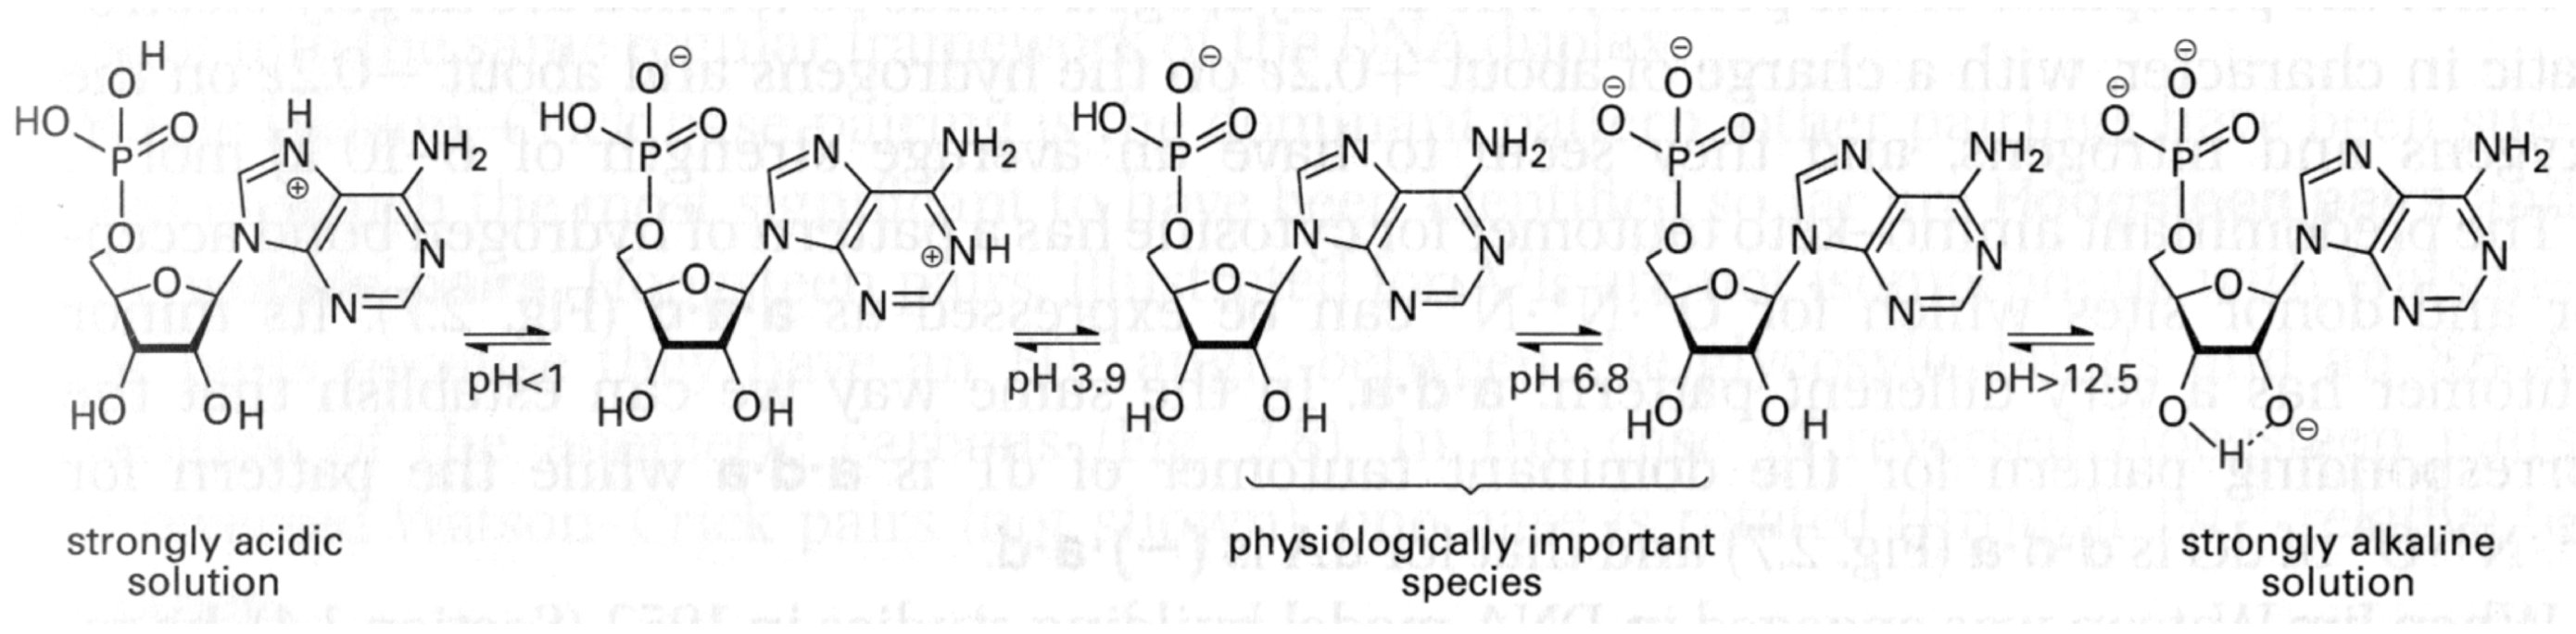
\includegraphics[width=0.9\linewidth]{../ExtFiles/dnaIonization.png}
        \caption{DNA ionization states.}
        \label{fig:dnaIonization}
    \end{figure}
    \begin{itemize}
        \item At physiological $\pH$ (5-9), only phosphates are charged (as desired).
        \item Phosphate $\pKa$s: About 1-2 and 7.
        \item Ribose with free $2'$ and $3'$ \ce{-OH} groups: $\pKa\approx 12.4$ (vs. 15-16 for an isolated secondary alcohol).
        \item Why are the heteroatoms on adenine that get protonated the ones that do?
        \item These numbers can change a lot after polymerization.
    \end{itemize}
    \item Anti and syn base conformations.
    \begin{itemize}
        \item We have free rotation about the glycosidic \ce{C^{1$'$}}-N bond, subject only to the whims of sterics.
        \item This leads to \textbf{anti} and \textbf{syn} conformations.
        \item Anti is preferred among natural nucleotides for steric reasons.
        \item Exceptions:
        \begin{itemize}
            \item G prefers syn in mononucleotides, in alternating CpGpCpG oligonucleotides, and in Z-DNA.
            \item Non-natural nucleotides can shift the equilibrium towards syn.
            \begin{itemize}
                \item Examples: 8-bromoguanosine (\ce{N^3} of the now-electron-deficient heterocycle seeks stabilization through an H-bonding interaction with the $5'$ hydroxyl group, but this requires a syn conformation to be most efficient [i.e., to bring the involved atoms close together]) and 6-methyluridine (Me is more bulky than \ce{=O}, so \emph{it} sits anti to the sugar).
            \end{itemize}
        \end{itemize}
    \end{itemize}
    \item \textbf{Bulk} (of the base): \ce{O^2} (the oxygen attached to the 2-carbon) in pyrimidines or the whole six-membered ring in purines.
    \begin{itemize}
        \item See Figure \ref{fig:baseNucleoside}.
    \end{itemize}
    \item \textbf{Anti} (base conformation): The bulk of the heterocycle points away from the sugar.
    \item \textbf{Syn} (base conformation): The bulk of the heterocycle is over the sugar.
    \item Base tautomerization basics.
    \begin{figure}[h!]
        \centering
        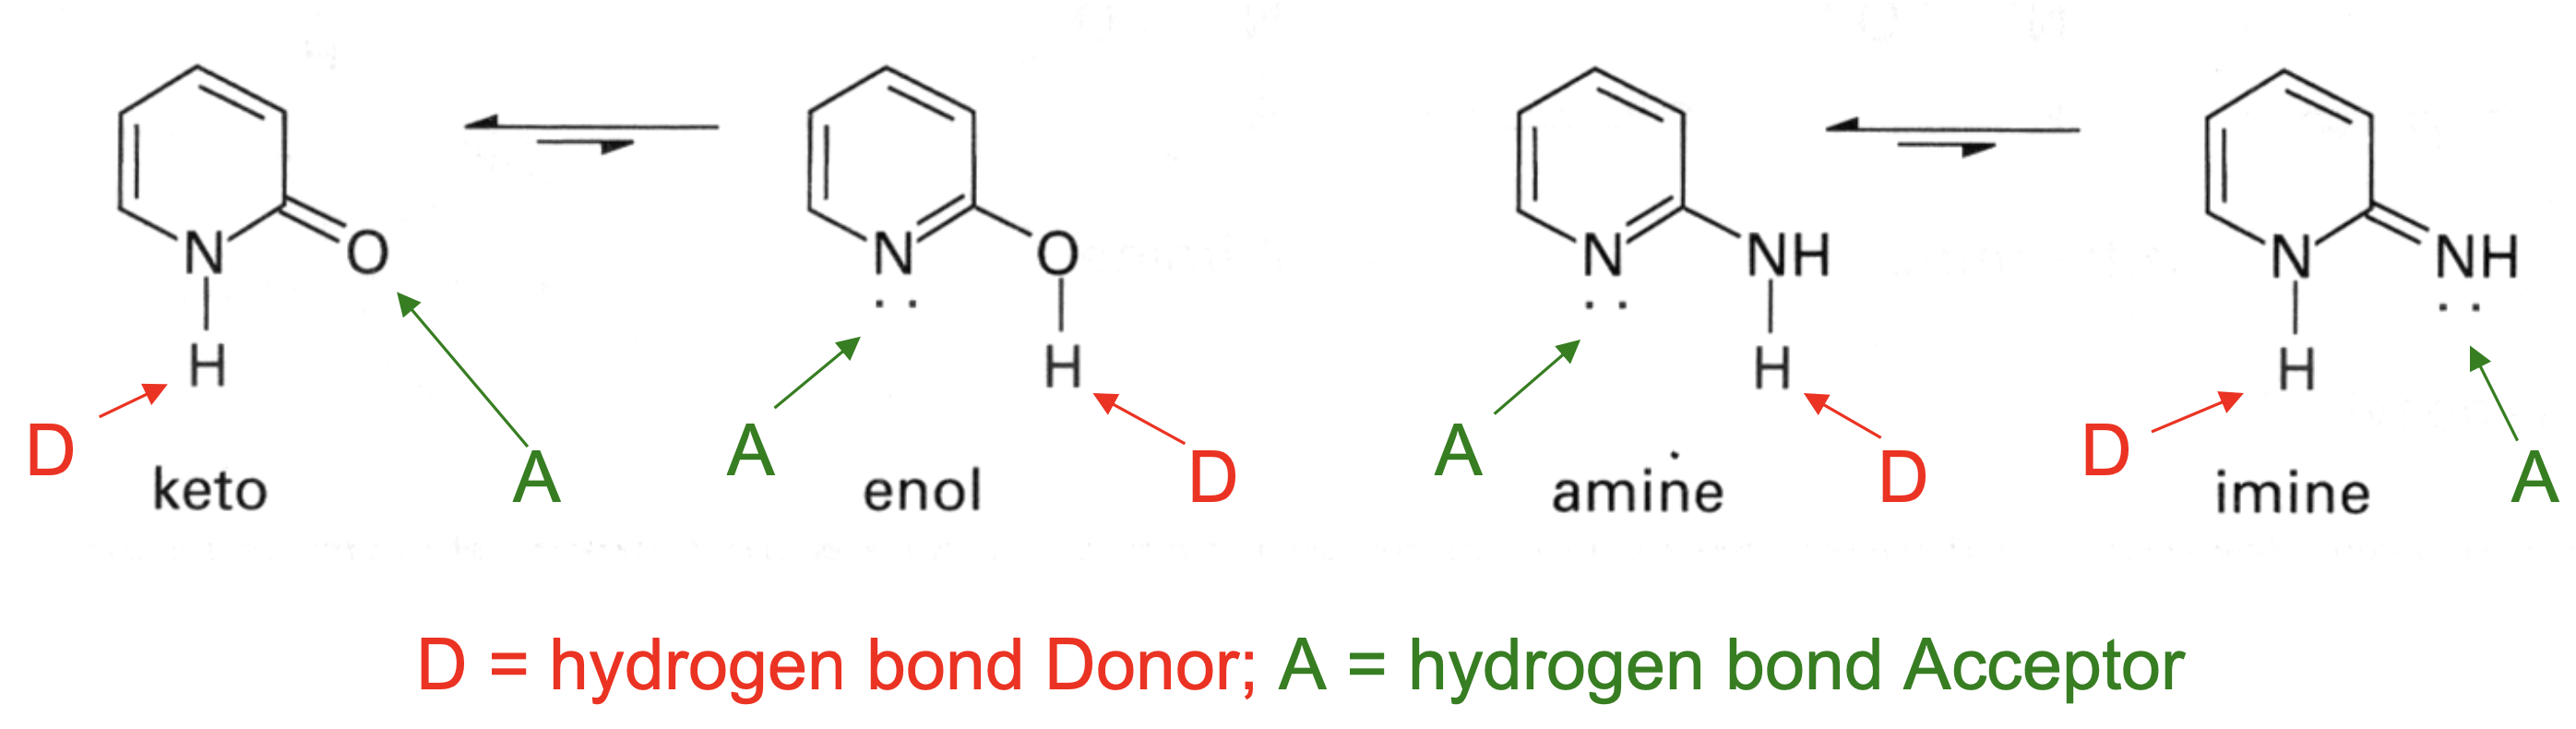
\includegraphics[width=0.7\linewidth]{../ExtFiles/baseTautomerization.png}
        \caption{Base tautomerization.}
        \label{fig:baseTautomerization}
    \end{figure}
    \begin{itemize}
        \item Recall that tautomerization involves movement in atoms whereas resonance does not.
        \item Bases exist in equilibrium between keto and enol forms, and between amino and imino forms.
        \item Tautomerization changes which groups function as hydrogen bond donors and acceptors in base pairing.
        \item The keto and amino forms among natural bases are preferred by more than $99.99\%$, according to X-ray and NMR analyses.
        \item It is difficult to determine what form a base is in just via organic chemistry first principles.
        \begin{itemize}
            \item Sometimes, tautomerization will do something highly unfavored like breaking aromaticity. But other times, making a system aromatic will generate an unstable enol. Confounding factors like this make it hard to tell.
            \item In fact, when Watson and Crick were originally solving the structure of DNA, they had it backwards until a physical chemist wrote to them with a calculation suggesting the right form, and that allowed Watson and Crick to solve the structure right away.
        \end{itemize}
    \end{itemize}
    \item Enol and imino tautomers lead to mutagenic H-bonding patterns.
    \begin{figure}[H]
        \centering
        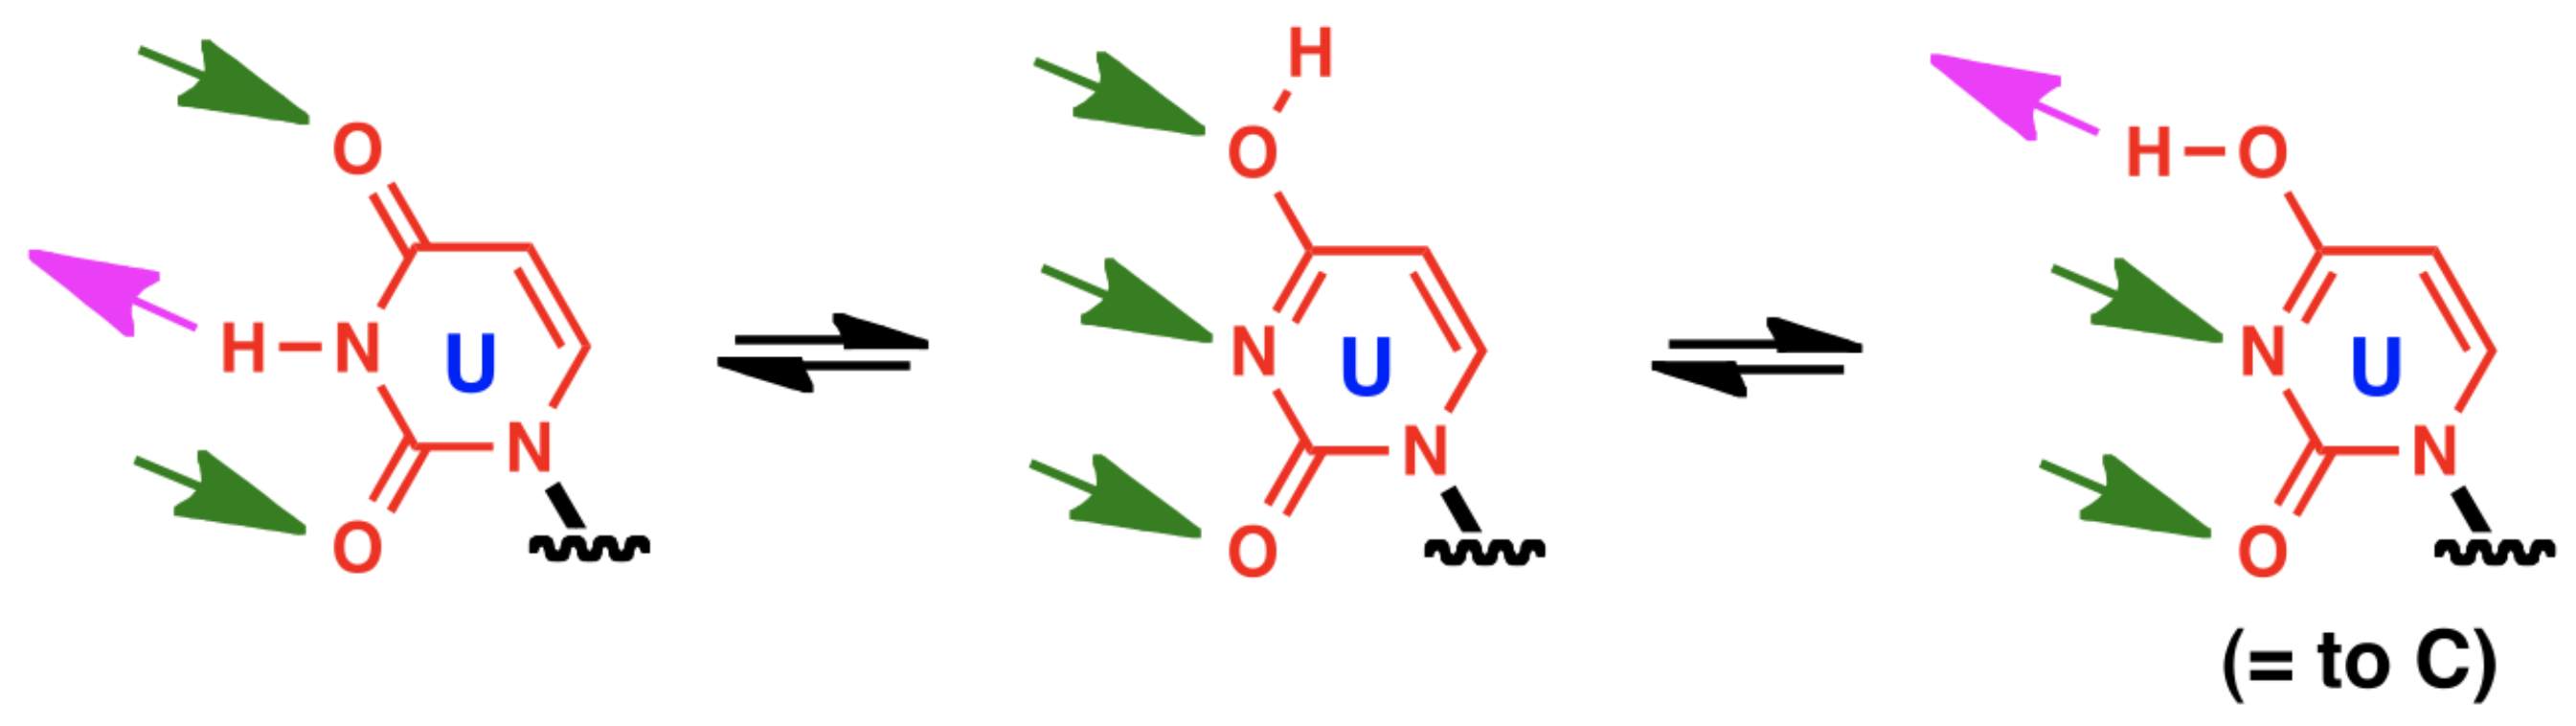
\includegraphics[width=0.6\linewidth]{../ExtFiles/uracilTautomerization.png}
        \caption{Uracil tautomerization.}
        \label{fig:uracilTautomerization}
    \end{figure}
    \begin{itemize}
        \item Because donor/acceptor dynamics are shifted, tautomers of one base can look like \emph{another} base from a hydrogen-bonding perspective.
        \item The tautomerization equilibrium can be shifted by functionalizing the base pairs. This is why bromine is a mutagen --- it makes it far more likely for U to be read as C, for instance.
        \item Tang goes over the tautomers for the other bases, too (see slides).
    \end{itemize}
    \item Ribose exists in many conformers.
    \begin{figure}[h!]
        \centering
        \begin{subfigure}[b]{0.2\linewidth}
            \centering
            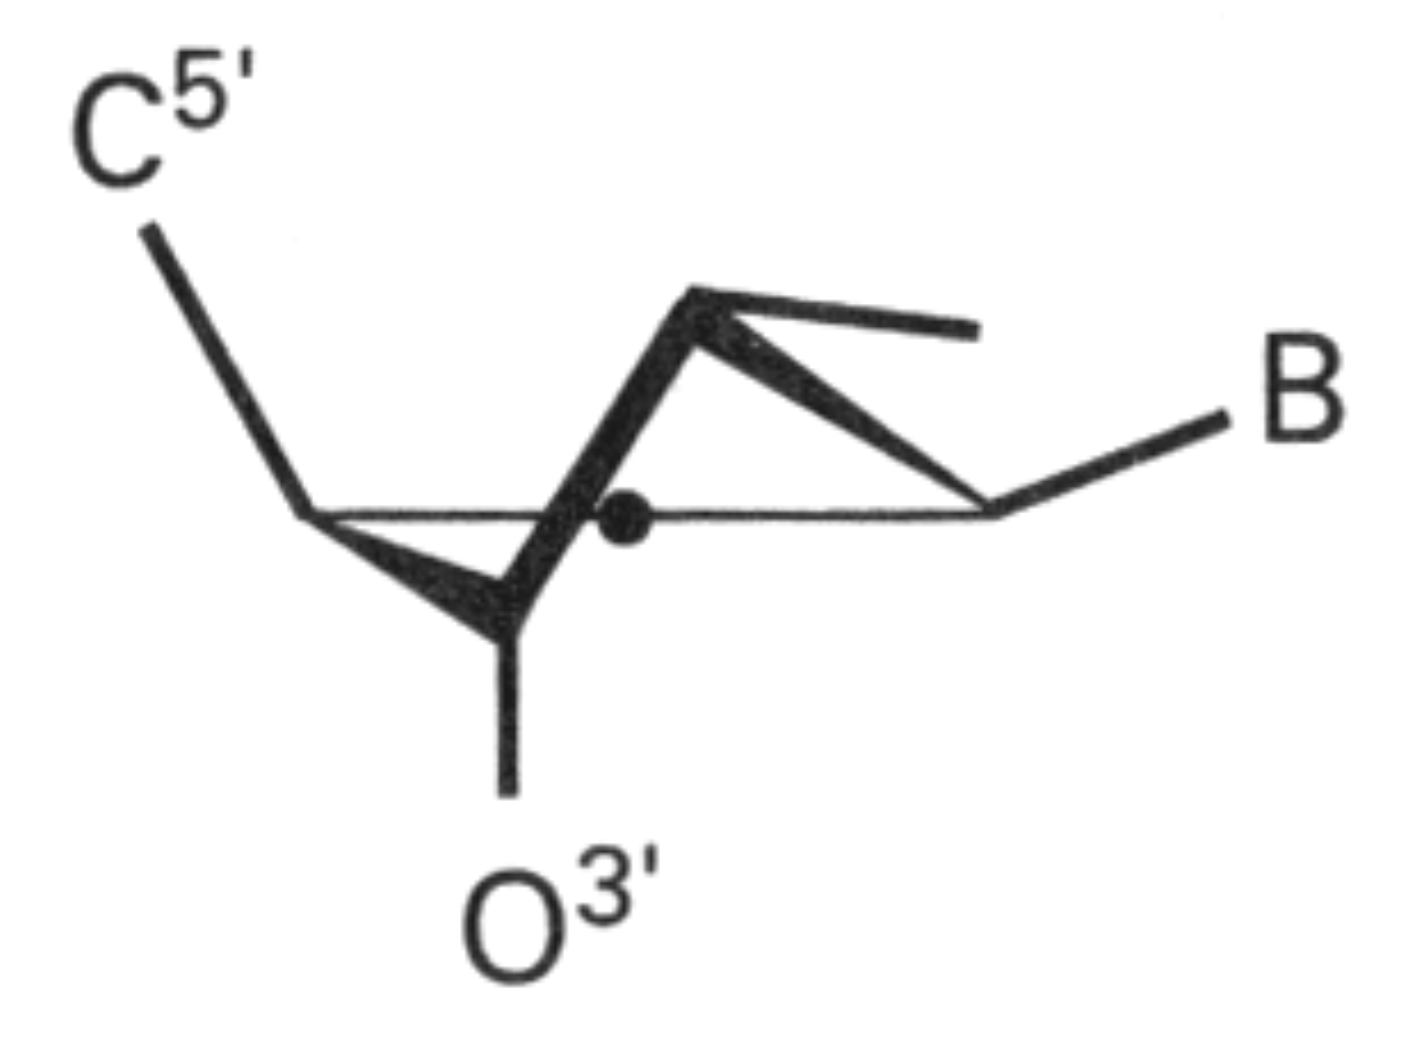
\includegraphics[width=0.8\linewidth]{../ExtFiles/puckomersa.png}
            \caption{\ce{C^{2$'$}}-\emph{endo}.}
            \label{fig:puckomersa}
        \end{subfigure}
        \begin{subfigure}[b]{0.2\linewidth}
            \centering
            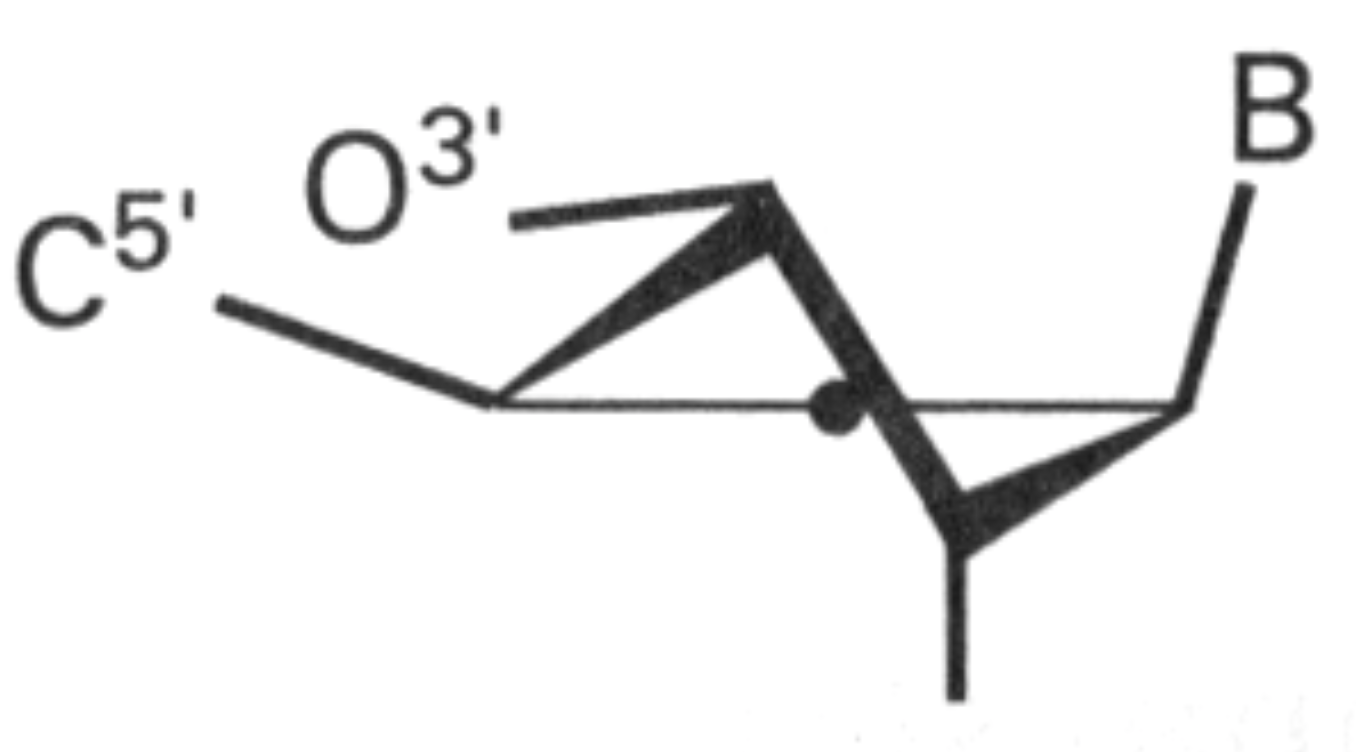
\includegraphics[width=0.8\linewidth]{../ExtFiles/puckomersb.png}
            \caption{\ce{C^{3$'$}}-\emph{endo}.}
            \label{fig:puckomersb}
        \end{subfigure}
        \caption{Puckomers of ribose.}
        \label{fig:puckomers}
    \end{figure}
    \begin{itemize}
        \item The furanose ring is nonplanar/puckered to minimize non-bonded interactions between substituents.
        \item \textbf{Endo} and \textbf{exo} atoms.
        \item \textbf{Puckomers} are in rapid equilibrium with an energy barrier of less than \SI[per-mode=symbol]{5}{\kilo\calorie\per\mole} (higher in polymeric DNA/RNA).
        \item Crystallography and NMR suggest two preferred puckomer groups: \ce{C^{2$'$}}-\emph{endo} and \ce{C^{3$'$}}-\emph{endo}.
        \begin{itemize}
            \item In the former, the $2'$-carbon of (deoxy)ribose is endo (and the $3'$-carbon exo; all others lie in the plane).
            \item In the latter, the $3'$-carbon of (deoxy)ribose is endo (and the $2'$-carbon exo; all others lie in the plane).
        \end{itemize}
        \item Sugar conformation dramatically changes the shape of the duplex.
        \begin{itemize}
            \item B-DNA favors \ce{C^{2$'$}}-\emph{endo} sugars.
            \begin{itemize}
                \item Since DNA runs $5'$ to $3'$, as we can see in Figure \ref{fig:puckomersa}, \ce{C^{2$'$}}-\emph{endo} gives us a more stretched out/relaxed form of the polymer. B-DNA is the most common form of DNA.
            \end{itemize}
            \item RNA and A-DNA favor \ce{C^{3$'$}}-\emph{endo} sugars.
            \begin{itemize}
                \item Conversely, \ce{C^{2$'$}}-\emph{endo} gives us a much more compact/bunched up form of the polymer.
            \end{itemize}
        \end{itemize}
    \end{itemize}
    \item \textbf{Endo} (atoms): Atoms on the same side of the furanose as \ce{C^{5$'$}}.
    \item \textbf{Exo} (atoms): Atoms on the opposite side of the furanose from \ce{C^{5$'$}}.
    \item \textbf{Puckomer}: A ribose conformer.
    \item Why RNA contains uracil and DNA contains thymine.
    \begin{itemize}
        \item There is a slow but appreciable rate of hydrolysis of C to U (500 times per cell per day).
        \item When C $\to$ U in DNA, because uracil is not a typical constituent of DNA and can easily be distinguished from T (T has an additional methyl group), our DNA correction mechanisms can easily repair the error, preventing our DNA from mutating long-term.
        \item RNA, on the other hand, cannot be edited. However, RNA is transient but DNA is not, and it is highly unlikely to have the same mutation at the same position every time. Thus, a few proteins are liable to get messed up in a variety of different ways from mutated mRNA, but long term, the base genetic code in DNA is preserved.
        \item Note that this is just a hypothesis (and a hard one to test), but it seems reasonable.
    \end{itemize}
    \item Why nature chooses phosphates.
    \begin{itemize}
        \item Requirements any possible linking group for nucleic acid monomers must satisfy.
        \begin{enumerate}
            \item Multivalent (so it can connect two monomers).
            \item Cannot cross biological barriers (e.g., the nuclear membrane).
            \item Kinetically stable to hydrolysis (we don't want our DNA strand to be breaking at random all the time).
            \item Thermodynamically unstable/must exist in high energy forms (we want the synthesis of the polymer [which involves cleaving some phosphate groups] to be thermodynamically favorable).
            \item Kinetically unstable with catalyst: modulated reactivity (so an enzyme can hydrolyze it; we don't want it to be so stable that we can't work with it).
        \end{enumerate}
        \item Phosphate groups satisfy these requirements since they\dots
        \begin{enumerate}
            \item Are divalent.
            \item Are polar.
            \item Are negatively charged (nucleophiles that might hydrolyze it are Coulombically repelled).
            \item Can exist in high energy forms (such as ATP).
            \item Are more reactive in the presence of magnesium.
        \end{enumerate}
        \item Some possible alternatives include citric acid, arsenate esters, silyl esters, and amides.
        \begin{itemize}
            \item Citric acid is abundant, but ester bonds are unstable in biological systems and the negative charges are quite far apart (so nucleophilic attack is not as hindered).
            \item Arsenate and silyl esters are also too labile.
            \item Amides are too stable; we can't hydrolyze it easily with any sort of catalyst.
            \begin{itemize}
                \item Scientists have used amides to connect nucleobases in the lab, though.
            \end{itemize}
        \end{itemize}
        \item This is another hard-to-test hypothesis that seems reasonable.
    \end{itemize}
    \item What binds two strands of DNA.
    \begin{itemize}
        \item Not hydrogen bonds.
        \begin{itemize}
            \item These only decide specificity; there is no thermodynamic preference for two-stranded DNA over single-stranded DNA hydrogen bonded unspecifically to a bunch of water molecules, for instance.
        \end{itemize}
        \item Stacking, on the other hand, is key.
        \begin{itemize}
            \item It excludes water and maximizes van der Waals interactions.
            \item More explanation?
            \item Not testable material.
        \end{itemize}
    \end{itemize}
    \item DNA and the double helix.
    \begin{itemize}
        \item DNA can occur in different 3D forms.
        \item Nucleic acids in higher order structures (e.g., tRNA and G-quadruplex).
        \item Geometric parameters.
    \end{itemize}
    \item DNA and RNA polymorphism.
    \begin{itemize}
        \item Various forms exist and are interchangeable; we don't need to know most of them.
        \item Determinants of DNA and RNA forms.
        \begin{enumerate}
            \item Sequence (not only composition).
            \item Counter ion and [salt].
            \item Humidity (crystals).
            \item Temperature.
        \end{enumerate}
        \item Not testable material.
    \end{itemize}
    \item Major nucleic acid forms.
    \begin{itemize}
        \item We are responsible for A-DNA, B-DNA, and Z-DNA.
        \begin{itemize}
            \item A- and B-DNA are most important; then Z-DNA.
        \end{itemize}
        \item A- and B-DNA are right-hand double helices; Z-DNA is a left-hand double helix.
        \item The number of base pairs per turn of\dots
        \begin{itemize}
            \item A-DNA is 11;
            \item B-DNA is 10;
            \item Z-DNA is 12.
        \end{itemize}
        \item The rise per base pair of\dots
        \begin{itemize}
            \item A-DNA is \SI{2.9}{\angstrom};
            \item B-DNA is \SIrange{3.3}{3.4}{\angstrom};
            \item Z-DNA is \SI{3.7}{\angstrom}.
        \end{itemize}
        \item Other important numbers?
        \item In B-DNA, the base pairs are relatively centered within the strand; in A-form, they rotate around.
    \end{itemize}
    \item B-DNA.
    \begin{itemize}
        \item Base pairs on center of helical axis.
        \item Major and minor is an accurate descriptor.
        \begin{itemize}
            \item What are these grooves and what is their significance?
        \end{itemize}
        \item Both grooves have similar depths.
        \item Sugar pucker is \ce{C^{2$'$}}-\emph{endo} ($2'$ and $5'$ on the same side).
    \end{itemize}
    \item A-DNA.
    \begin{itemize}
        \item Base pairs are displaced from center of helical axis.
        \item Major groove less wide than minor.
        \item Sugar pucker is \ce{C^{3$'$}}-\emph{endo} ($3'$ and $5'$ on the same side).
        \item DNA/RNA hybrids are A-like (transcription, reverse transcription, and DNA replication).
    \end{itemize}
    \item Enzymes recognize the 3D helical structure of DNA, not just their individual substrate. Like reading a word instead of letter by letter.
    \item Higher order structures.
    \begin{itemize}
        \item The structure of tRNA provides a wealth of information.
        \begin{itemize}
            \item Until the early 1990s, we could only crystallize tRNA, so we primarily learned from it for a long time.
        \end{itemize}
        \item L-shape: Two perpendicular A-RNA helices.
        \item Tons of fun H-bonding interactions provide structure. Even three nucleobases can interact all together in some cases.
    \end{itemize}
    \item G-quadruplex.
    \begin{figure}[h!]
        \centering
        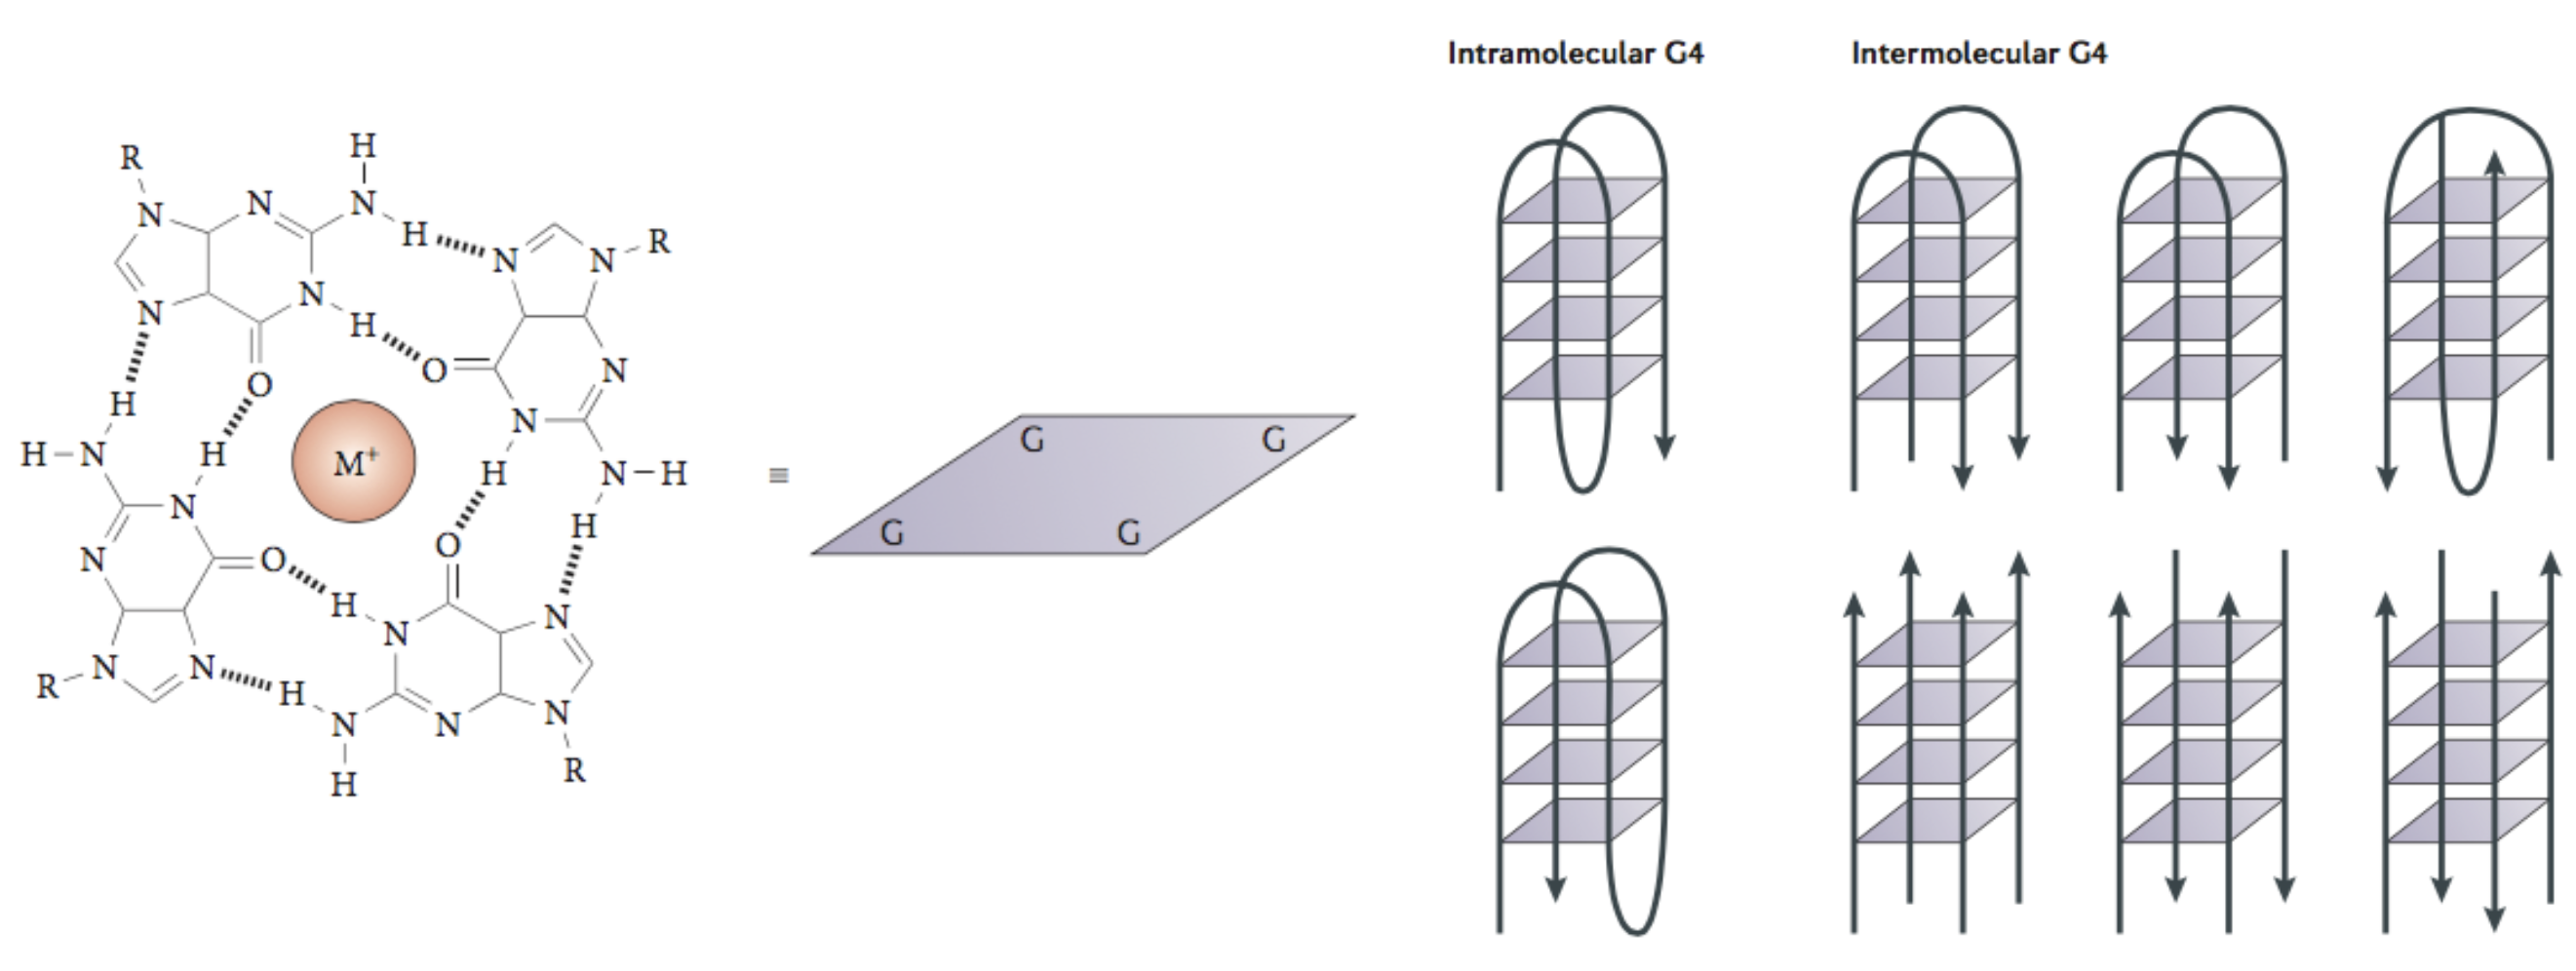
\includegraphics[width=0.9\linewidth]{../ExtFiles/gQuadruplex.png}
        \caption{G-quadruplex structure.}
        \label{fig:gQuadruplex}
    \end{figure}
    \begin{itemize}
        \item Helical structure containing guanine tetrads from one, two, or four strands.
        \item Hoogsteen hydrogen bonding.
        \item Stabilized by the presence of a cation, especially potassium.
        \item Importance of G-quadruplexes.
        \begin{itemize}
            \item Chromosomes have a structure called a telomere at both ends. During replication, some of the telomere is lost each time. When the whole telomere is gone, the cell will not be able to divide any more. This is the aging process, and the discovery of telomeres received the Nobel prize in the early 2000s.
            \item Telomerase is an enzyme that fights against this loss, trying to extend the DNA post-replication using RNA templates.
            \item If telomerase is overactivated, the cells are immortalized and they become cancerous.
            \item Telomeric quadruplexes decrease the activity of telomerase; they moderate telomerase so that it's active enough so that we don't die early, but not so active that we become big balls of cancer.
        \end{itemize}
    \end{itemize}
    \item The spinach aptamer.
    \begin{itemize}
        \item For a long time, we've been able to tag any \emph{protein} we want with GFP (green fluorescent protein) and follow it.
        \item It would be very beneficial to be able to do the same thing with RNA.
        \item Thanks to the Jaffrey lab, now we can with DFHBI.
        \item The spinach aptamer binds to DFHBI and becomes fluorescent in the presence of RNA. DFHBI's $\pi$ structure too bendy to flouresce on its own, but when it is stabilized by insertion into RNA, it can fluoresce.
        \item We still need a lot of work before this is as good as GFP.
    \end{itemize}
    \item The remaining slides will be covered next lecture.
\end{itemize}




\end{document}